\documentclass[a4paper,12pt]{article}
\usepackage[utf8]{inputenc}
\usepackage[T2A]{fontenc}
\usepackage[russian,english]{babel}
\usepackage[pdftex]{graphics}
\DeclareGraphicsExtensions{.pdf,.png,.jpg}
\graphicspath{{pictures/}}
\begin{document}
\begin{center}
Санкт-Петербургский государственный политехнический университет
\\Кафедра компьютерных систем и программных технологий
\end{center}
\vspace*{10em plus .6em minus .5em}

\begin{center}
{\LARGEТелекоммуникационные технологии
\\Лабораторная работа №8
\\Цифровая модуляция}
\end{center}

\vspace*{5em plus .6em minus .5em}
\begin{flushright}
Выполнил:\\студент гр.33501/4\\Корсков Алексей\\Проверила:\\Богач Н.В.
\end{flushright}

\vspace*{15em plus .6em minus .5em}
\begin{center}
{\smallСанкт-Петербург
\\2018}
\end{center}
\pagestyle{empty}
\newpage
\pagestyle{plain}
{\bfseriesЦель}

Создать модель телекоммуникационного канала.

{\bfseriesПостановка задачи}

Задача: по имеющейся записи сигнала из эфира и коду модели передатчика создать модель приемника, в которой найти позицию начала пакета и, выполнив операции демодуляции, деперемежения и декодирования, получить передаваемые параметры: ID, период, и номер пакета. Известно, что ID = 4, период 100 мс, номер пакета 373. Запись сделана с передискретизацией 2, т.е. одному BPSK символу соответствуют 2 лежащих друг за другом отсчета в файле. Запись сделана на нулевой частоте и представляет из себя последовательность 32-х битных комплексных отсчетов, где младшие 16 бит вещественная часть, старшие 16 бит – мнимая часть.

{\bfseriesТеоретическое обоснование}

Пакетный сигнал длительностью 200 мкс состоит из 64 бит полезной информации и 8 нулевых tail-бит. В нулевом 16-битном слове пакета передается ID, в первом - период излучения в мс, во втором – сквозной номер пакета, в третьем - контрольная сумма (CRC-16). На передающей стороне пакет сформированный таким образом проходит следующие этапы обработки:

\begin{enumerate}

\item Помехоустойчивое кодирование сверточным кодом с образующими полиномами 753, 561( octal ) и кодовым ограничением 9. На выходе кодера количество бит становится равным 144.
\item Перемежение бит. Количество бит на этом этапе остается неизменным.
\item Модуляция символов. На этом этапе пакет из 144 полученных с выхода перемежителя бит разбивается на 24 символа из 6 бит. Генерируется таблица функций Уолша длиной 64 бита. Каждый 6-битный символ заменяется последовательностью Уолша, номер которой равен значению данных 6-ти бит. Т.о. на выходе модулятора получается 24 * 64 = 1536 знаковых символов.
\item Прямое расширение спектра. Полученная последовательность из 1536 символов периодически умножается с учетом знака на ПСП длиной 511 символов. Далее к началу сформированного символьного пакета прикрепляется немодулированная ПСП. Т.о. символьная длина становится равной 1747. Далее полученные символы модулируются методом BPSK.
\end{enumerate}
\newpage

{\LargeХод работы}
\begin{enumerate}
{\item
\center{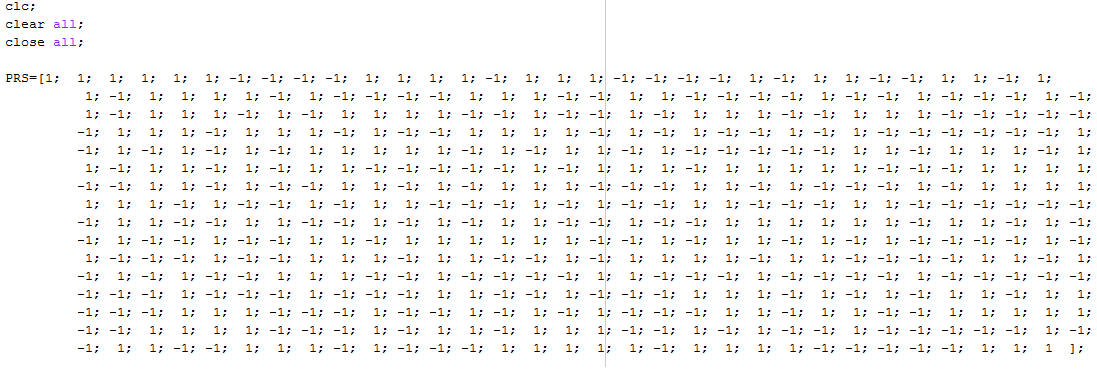
\includegraphics{./pictures/pic1.png} \\ Рис.1 Результат работы программы}
\\}

{\item
\center{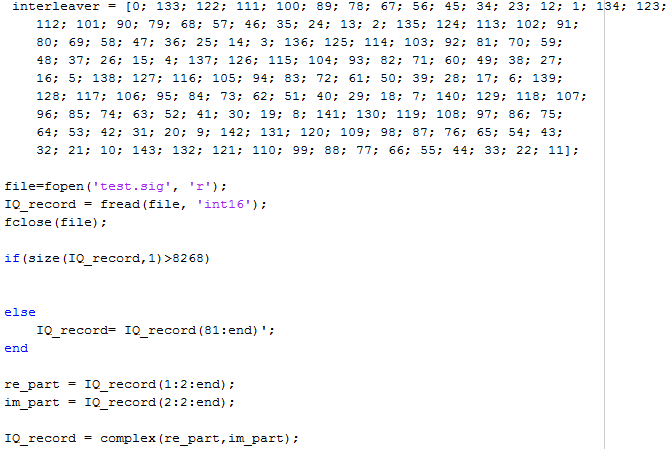
\includegraphics{./pictures/pic2.png} \\ Рис.2 Результат работы программы}
\\}

{\item
\center{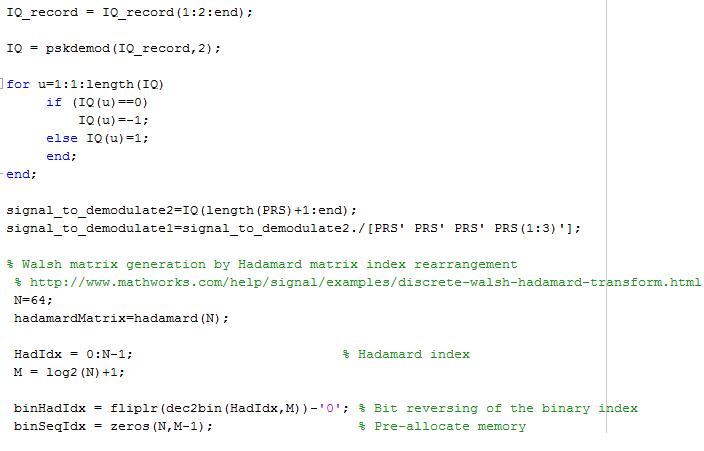
\includegraphics{./pictures/pic3.png} \\ Рис.3  Результат работы программы}
\\}

{\item
\center{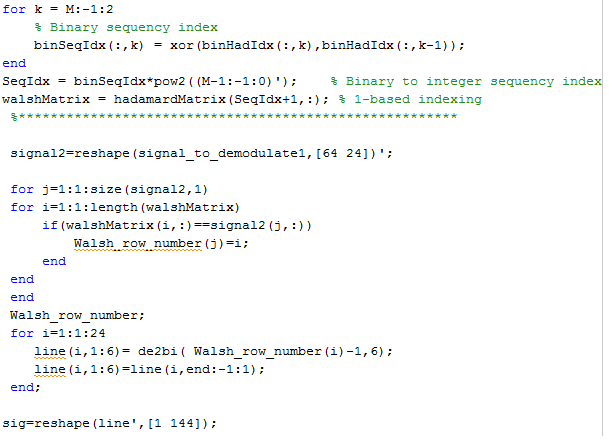
\includegraphics{./pictures/pic4.png} \\ Рис.4 Результат работы программы}
\\}

{\item
\center{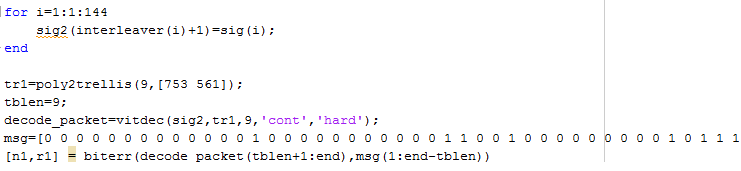
\includegraphics{./pictures/pic5.png} \\ Рис.5 Результат работы программы}
\\}

{\bfseries\LARGEВывод}

В ходе данной работы было разработано, промоделировано, отлажено и настроено устройство приема данных согласно конкретному техническому заданию. 

Модель приемника была создана на основе модели передатчика: были проведены обратные действия. Когда на передатчике были проведены операции модуляции, перемежения и кодирования параметров, на приемнике были выполнены демодуляциия, деперемежение и декодирование, были получены передаваемые параметры.

\end{enumerate}
\end{document}
